\chapter{Background}
\label{chapter:background}

This chapter delineates a general overview of multiphysics simulation, coupling tool, and co-simulation process. This research majorly focuses on FSI interaction studies to test the research hypothesis- automated algorithm configurations can effectively configure coupling tool parameters. Therefore, FSI simulations are introduced, and the use-cases are discussed. In addition, the chapter explains automated algorithm configuration and mathematically formulates the problem in the final section.

\section{Multiphysics simulation}
Multiphysics simulation is the process of simulating the interaction of various physical phenomena involving multiple physical domains. Multiphysics simulation tools aid in modeling the physical processes with a set of mathematical formulas and studying the behavior in a software interface. There are various categories of multiphysics simulations, depending on the physical processes under study. A few categories are FSI, heat transfer, structural mechanics, fluid flow, hydrostatics, chemical reactions, acoustics, and magnetostatics \cite{FSI_Bungartz}.

The examples below are the results of the multiphysics simulation. Figure \ref{Fig:car-acoustics} illustrates the distribution of the acoustic pressure field in Pascal(Pa) across a car with the sound source at the speaker. This study helps the user to optimize the speaker location depending on the mirror sources and damping factors \cite{car-acoustics}.

\begin{figure}[!ht]
\centering
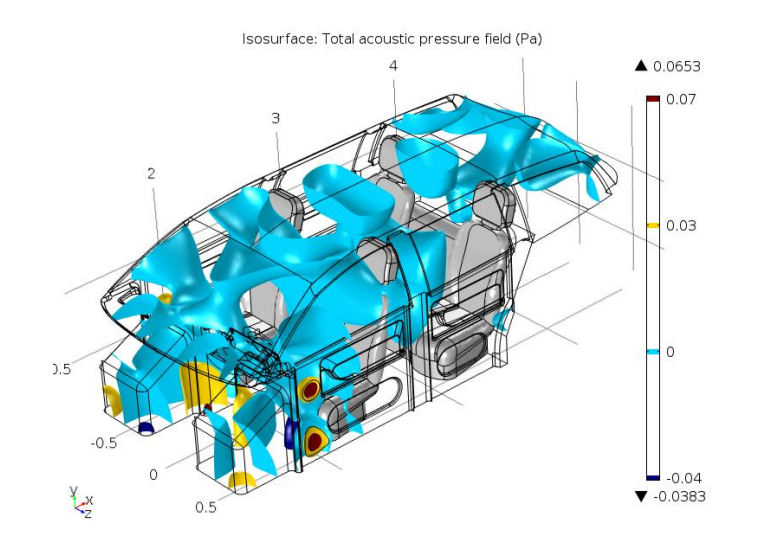
\includegraphics[width=\textwidth]{images/car-acoustics.png}
\captionsetup{justification=justified}
\caption[Multiphysics simulation example- Acoustic field study of a car]{Total acoustics pressure field in Pascal (Pa)- Acoustics field study of a car \cite{car-acoustics}.}
\label{Fig:car-acoustics}
\end{figure}

The figure \ref{Fig:submarine} is a simulation to study the magnetic signature of a submarine traveling underwater. The study is vital in designing naval ships because the submarine traveling underwater disturbs the Earth's magnetic field and potentially triggers weapons. In addition, the study of magnetic signatures is imperative to design navigational control units, and magnetic grippers \cite{submarine}. The figure \ref{Fig:submarine} shows the distribution of magnetic flux density, Tesla (T) of a submarine underwater with the arrows representing the tangential magnetic flux density \cite{submarine}.

\begin{figure}[!ht]
\centering
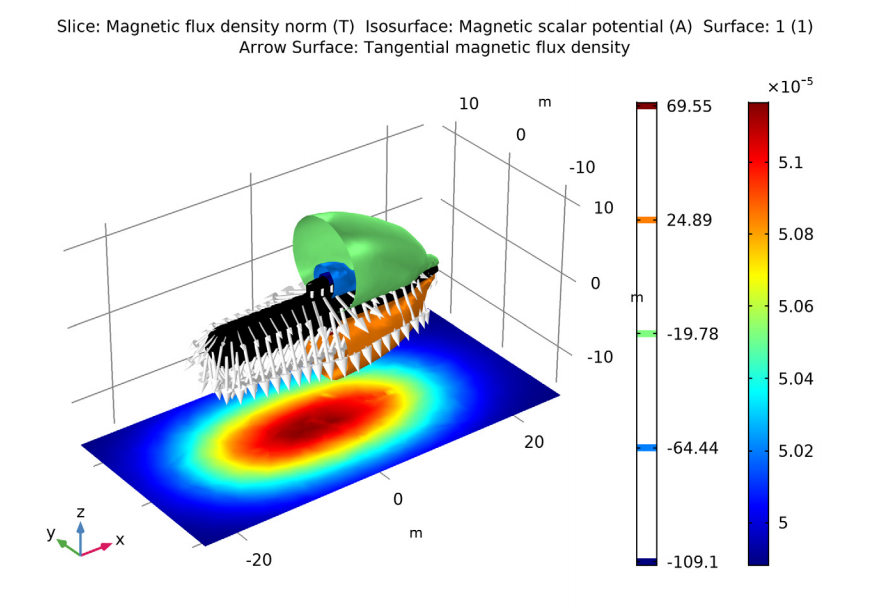
\includegraphics[width=\textwidth]{images/submarine.png}
\captionsetup{justification=justified}
\caption[Multiphysics simulation example- Magnetic flux study of a submarine]{Total magnetic flux density in Tesla (T) of a submarine in an ocean \cite{submarine}.}
\label{Fig:submarine}
\end{figure}

% \subsection{Multiphysics simulation solution approaches}

% Multiphysics simulations are carried out in two approaches namely monolithic and partitioned coupling \cite{Couplingenv_Gatzhammer}.

% In monolithic approach, the mathematical model governing all the domain characteristics and interactions among different domains is developed in a single complex model and discretized to solve the model. Though this method aids to control error and improve robustness, managing each individual parameters is highly difficult \cite{FSICartesiangrid}.

% In partitioned coupling simulation, the physical fields are solved individually. However, both domains share specific variables and necessitates data sharing between the domains. This data sharing and solving the governing equations generic to both domains is carried out in the coupling region. This kind of multiphysics  systems are known as coupled systems \cite{MpCCI_documentation}.

% The coupling process is carried out in a coupling tool called coupling environment or coupling software. The various coupling environments are Mesh-based parallel Code Coupling Interface (MpCCI), Fluid-Structure Interaction Coupling Environment (FSI❄ce), preCICE, JADE, ADVENTURE\_Coupler, MUSE, etc., \cite{Couplingenv_Gatzhammer}.

% One of the most important concepts in partitioned simulation is the type of coupling and the method of variable sharing between the domains. The variables of all the domains and coupling parameters are utilized by the solver for studying the interaction between each domain and the properties of the entire system.

% For instance, in Fluid-Structure Interactions (FSI) the variable related to pressure and displacement are shared between the domains for solving the system. This process of sharing data between the domains is called coupling \cite{MpCCI_documentation}.

% The advantages of partitioned coupling of multiphysics simulation in a coupling environment:
% \begin{itemize}
% \item The coupling environment fosters in code re-usability by maintaining separate solver and mathematical models for each domain. The domain specific solvers and source codes pertaining to the domain can be combined to solve a complex multiphysics simulation in the coupling environment \cite{Couplingenv_Gatzhammer} \cite{FSICartesiangrid}.

% \item This reduces the complexity in developing a complex mathematical model considering all the physical aspects of the multiple domains in the study. For instance, fluid domain and solid structural domain mathematical models \cite{Couplingenv_Gatzhammer} \cite{FSICartesiangrid}.

% \item This decreases the cycle time for implementation and maintenance of a new complex code for solving various multiphysics simulations.

% \item In addition, this method of coupling the multiple domains independent of the specific physical properties in a coupling environment helps in experimenting with the optimal solution. The experiment is established by switching the sub-fields of the physical domains, simulating with different solvers and models. Cumulatively, partitioned simulation in a coupling environment enhances the flexibility and scalability of the multiphysics simulations \cite{Couplingenv_Gatzhammer} \cite{FSICartesiangrid}.
% \end{itemize}

\subsection{Fluid-Structure Interaction (FSI)}

FSI is one of the multiphysics simulations. In FSI, a deformable solid structure interacts with a compressible or incompressible fluid flow, where pressure and displacement are the coupled quantities. The two domains of an FSI simulation are the fluid and solid domains. The fluid and solid domains are governed by fluid flow principles and solid mechanics principles, respectively. Figure \ref{Fig:Fluid-Structure-example} illustrates an FSI model. The model aids in understanding the flow of the fluid inside a rigid wall with a flexible flap protruding between the walls. The flap opens and closes depending on the fluid flow direction. In addition, the simulation helps to examine the behavior of a valve with regards to the outlet and inlet fluid pressure. The coupling region is clearly depicted in the left-hand side of the figure \ref{Fig:Fluid-Structure-example} coupling the flap surface and the fluid. 
\begin{figure}[!ht]
\centering
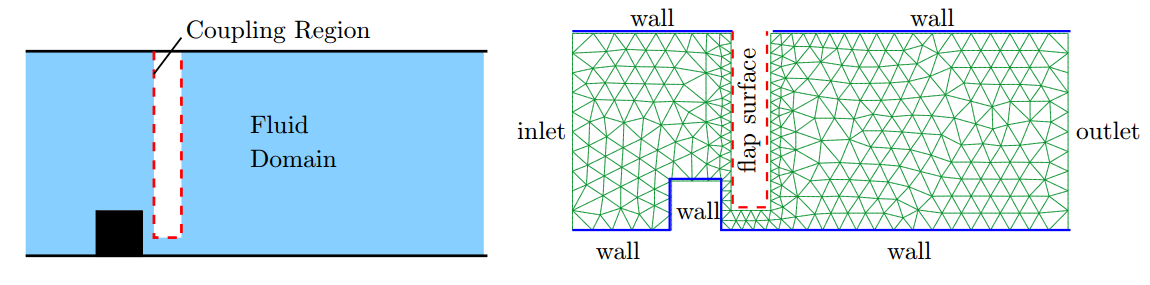
\includegraphics[width=\textwidth]{images/Fluid-Structure-example.png}
\captionsetup{justification=justified}
\caption[An example of Fluid-Structure Interaction model]{An example of Fluid-Structure Interaction model \cite{MpCCI_documentation}.}
\label{Fig:Fluid-Structure-example}
\end{figure}

The other examples of multiphysics simulation are thermomechanical couplings involving solid mechanics and heat conduction \cite{MpCCI_documentation}, and electrothermal couplings involving electrical conduction and heat conduction \cite{MpCCI_documentation}. This project significantly focuses on the FSI multiphysics simulation. 

\subsubsection{Use-cases of FSI}
\label{section:use-cases}
A few applications of multiphysics simulations can be witnessed in automobiles, aircraft, robotics, and life sciences industries.
\begin{itemize}

\item \textbf{Automobile:} The figure \ref{Fig:F1} illustrates the motion of the F1 car through the air in a simulated environment. This is used to design the F1 cars efficiently with optimal fuel consumption and reduce the drag on the car by the airflow.

\begin{figure}[!ht]
\centering
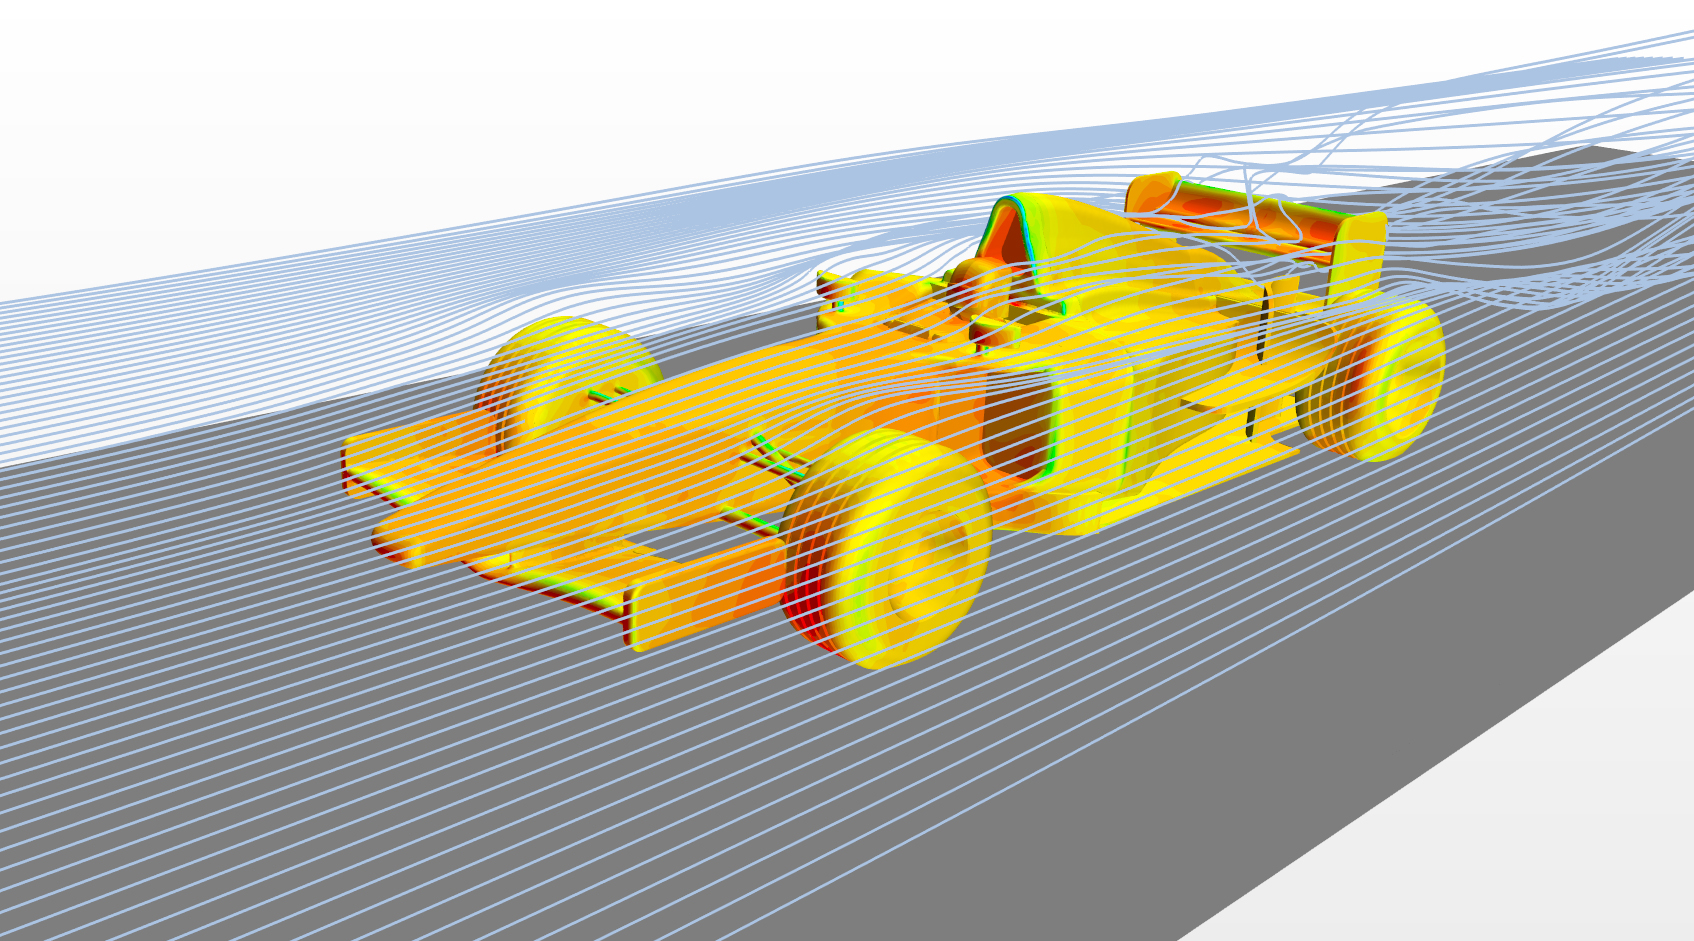
\includegraphics[width=0.8\textwidth]{images/f1_illustration.jpg}
\captionsetup{justification=justified}
\caption[Aerodynamics simulation study of F1 cars]{Aerodynamics simulation study of F1 cars \cite{MpCCI_documentation}.}
\label{Fig:F1}
\end{figure}

\item \textbf{Aircraft:} Multiphysics simulations are used to study the aerodynamics of aircraft and understand the drag caused on the aircraft during the motion.

% , as shown in figure \ref{Fig:aircraft}.

% \begin{figure}[!ht]
% \centering
% 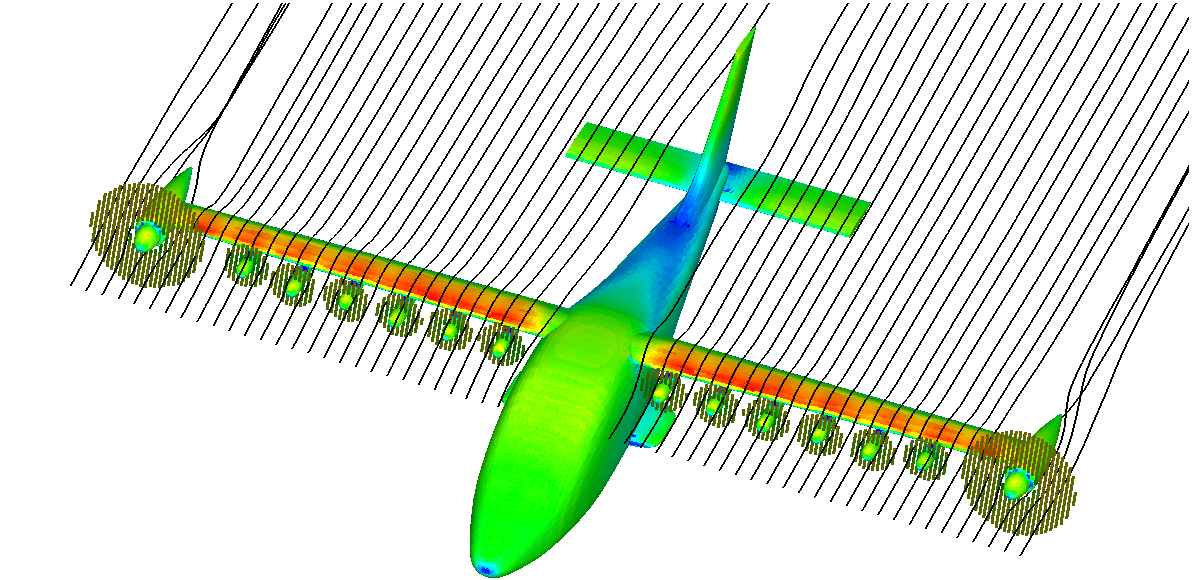
\includegraphics[width=\textwidth]{images/aeroplane_illustration.png}
% \captionsetup{justification=justified}
% \caption[Aerodynamics simulation study of aeroplanes]{Aerodynamics simulation study of aeroplanes \cite{aeroplane_image}.}
% \label{Fig:aircraft}
% \end{figure}
\item \textbf{Robotics:} Robots are widely used in domestic and industrial applications. In all these applications, the solid surfaces of the robots are in contact with air, water, or solid. Multiphysics simulations are carried to study the interaction of the robot surfaces with the environment and efficiently design the body of the robot \cite{Robots_applications}.

\item \textbf{Life sciences:} In life sciences, simulations play an integral role in studying the interaction of artificial organs with blood and motion of blood in a blood vessel \cite{Blood-vessel}. The figure \ref{Fig:Blood-vessel} is the output of a multiphysics simulation study. The study investigates the aorta, the blood vessel carrying blood to all parts of the body from the heart. The figure \ref{Fig:Blood-vessel} illustrates the displacement of the artery walls due to the pressure exerted by the blood flow.
\begin{figure}[!ht]
\centering
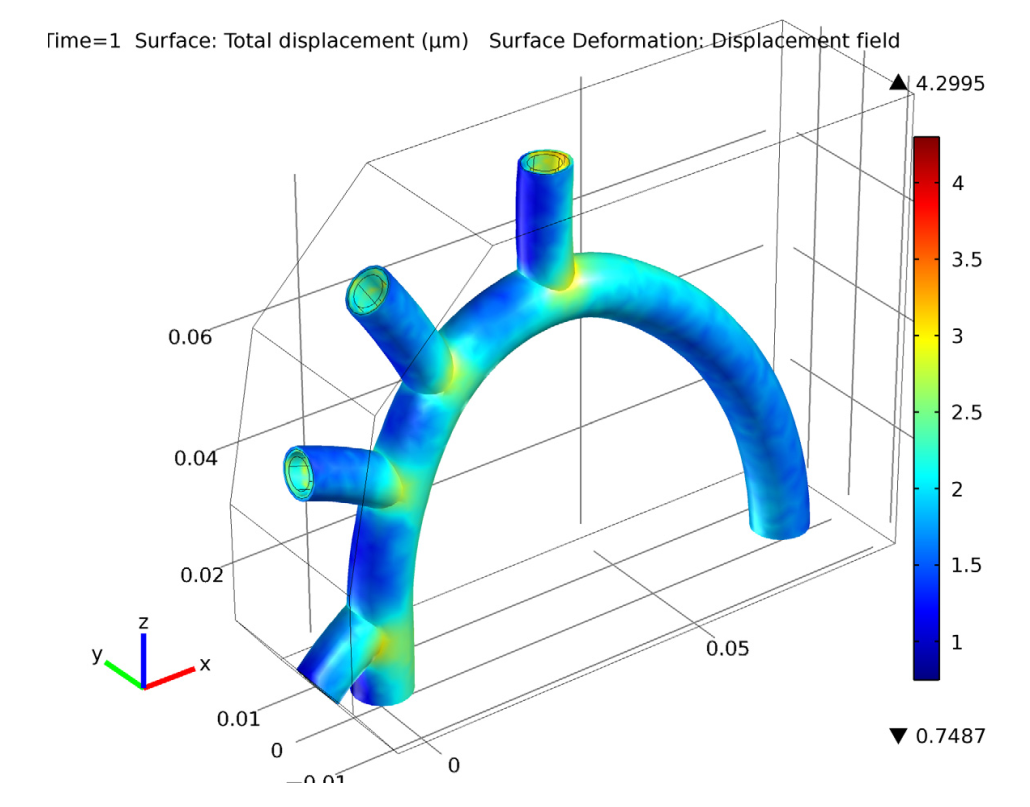
\includegraphics[width=\textwidth]{images/blood-vessel.png}
\captionsetup{justification=justified}
\caption[Displacement in the blood vessel due to blood flow]{Displacement in the blood vessel due to blood flow \cite{Blood-vessel}.}
\label{Fig:Blood-vessel}
\end{figure}
\end{itemize}

\subsection{Parameter types of a co-simulation process}
Multiphysics simulations are performed by a multiphysics simulation tool. The simulation code and the coupling environment are the integral components of the multiphysics simulation tool. The computer understandable instructions of the physical domain properties, physical processes, and the equations governing the mathematical model of the processes are called the simulation code. The physical phenomena are heat transfer, hydrodynamics, aerodynamics, chemical reactions, and solid mechanics. The simulation codes are specific to each domain involved in the study. The examples of simulation codes or solvers are ANSYS Fluent, OpenFoam, and ABAQUS.

 The coupling environment or the coupling tool is a computer program performing data communication between the simulation codes, data post-processing, and visualization of the simulation results, as illustrated in figure \ref{Fig:Couplingoverview}. The user sets up the simulation code depending on the study requirements. 
 
 Multiphysics simulations incorporate parameters and variables. The parameters define the characteristic of simulation, and on changing the parameters, the simulation behavior changes. The behavioral changes of a simulation impact the accuracy and time taken to complete the simulation. Most of the parameters are fixed over the entire simulation period. However, a few parameters change depending on the complexity and requirements of the study. A variable represents a particular state of a model and serves as a placeholder to store data. 
\afterpage{ 
\begin{figure}[!ht]
\centering
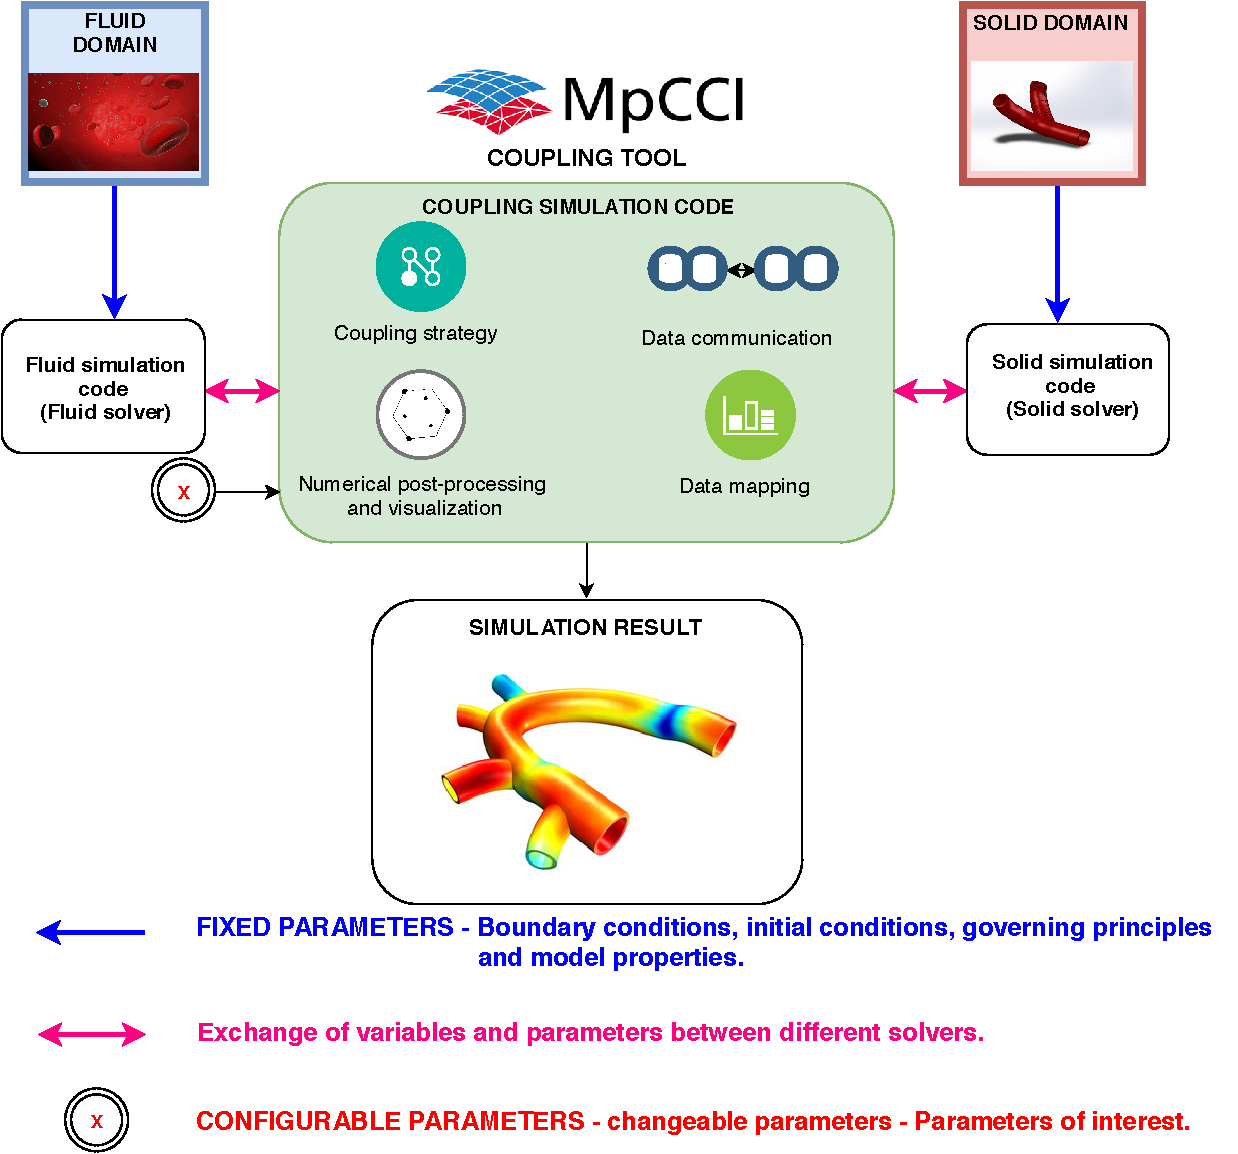
\includegraphics[width=0.9\linewidth,height=0.7\textheight]{images/Coupled_simulation.pdf}
\captionsetup{justification=justified}
\caption[Multiphysics simulation of a coupled system]{Multiphysics simulation of a coupled system. The color gradient in the simulation result represents the displacement profile of the blood vessel due to blood flow\footnotemark.}
\label{Fig:Couplingoverview}
\end{figure}
\footnotetext{The image provided inside the rectangular boxes- simulation result, fluid domain, and solid domain are from \cite{Blood-vessel} \cite{blood} \cite{vessel}.}
}
 
 The simulation studies include two types of parameters, namely fixed parameters and configurable parameters.
 
 \begin{itemize}
     \item \textbf{Fixed parameters:} The fixed parameters are attributed from three sources, namely the solid simulation code, fluid simulation code, and the coupling tool. The fixed parameters of the simulation codes include the simulation models and equations related to the physical process under study. The coupling environment includes a few study condition parameters such as coupled region, coupled variables, tolerance of the study, and the number of iterations. The fixed parameters of a simulation are specific to a particular simulation study performed by the user.
     
     \item \textbf{Configurable parameters:} The parameters concerning the coupling behaviour are configurable by the user in the coupling tool. The configurable parameters of the coupling tool are the hyperparameters of the coupling tool because the parameters can be tuned to control the simulation time and simulation accuracy. On tuning the configurable parameters manually, the performance of the simulation study largely differ. The examples of configurable parameters are the time step of the simulation, coupling method, relaxation method, and constants of the coupling strategy. A detailed explanation of the parameters is provided in section \ref{section:hyperparameters_couplingtool}.
 \end{itemize}
 
The figure \ref{Fig:Couplingoverview} illustrates a multiphysics simulation process of blood flowing in a blood vessel. The blood vessel with blood flow is the coupled system incorporating FSI physics. The coupling tool communicates the data in a particular manner between the solid and fluid solver over the entire course of the simulation. In this study, MpCCI, a coupling tool, is used to perform multiphysics simulations through the partitioned coupling. The configurable parameters set by the user in the coupling tool are the parameters of interest. 


\section{Automated Algorithm Configuration (AAC)}

The algorithms solving hard computations are prominently guided by a search strategy and are mostly parameterized. The tree search parameters include bounds at each level, the decision rule for branching, minimum nodes in the child branch, and depth \cite{SMAC_extendedpaper}. The search strategy pertaining to IBM ILOG CPLEX, one of the mixed-integer programming solvers, exposes 76 parameters. The parameters largely affect the solver performance, and manually examining the parameter space for best configuration is highly tedious \cite{SMAC_extendedpaper}. 
AAC approaches configure a target algorithm using parameter values that maximize a particular performance metric. The AAC methods are general-purpose configurators. On a training instance set, AAC methods estimate the optimal parameter configuration by optimization of the target algorithm. This process of tuning the parameters on a training set is called offline configuration. The best configuration is used to configure the algorithm in real-time \cite{SMAC_extendedpaper}. The applications of AAC includes AI planning \cite{AIplanning}, mixed integer programming \cite{ParamILS_mainpaper}, SAT solvers \cite{SAT_examplepaper}, and answer set programming \cite{ASP_solver}. In addition, AAC methods are extended to identify the optimum parameter configuration for machine learning frameworks \cite{Expertdown2} \cite{Robust_AutoML}, deep architectures and deep neural networks \cite{HPO_AC} \cite{AC_benchmarking}. An extended overview of the various state-of-the-art methods in AAC is provided in chapter \ref{chapter:stateoftheart}.

\subsection{A primer on Algorithm Configuration Problem (ACP)}

The problem of configuring the parameter of the coupling tool with optimal values is formulated using an Algorithm Configuration Problem (ACP). The algorithms optimizing the target algorithm performance are called configuration procedures or algorithm configurators. The formal definition of ACP is defined by, "given a parameterized target algorithm $\mathcal{A}$ with a set of instances $\Pi$ and parameter configuration space $\Theta$ with a cost metric 'c': $\Theta$ x $\Pi$ $\rightarrow$ $R$, the problem of estimating an optimal configuration $\theta$* $\in$ $\Theta$ by minimizing the cost metric over all the instances in $\Pi$" \cite{Pitfalls} \cite{AC_benchmarking}. 

\begin{equation}
    \theta^* \in \underset{\theta\in\Theta}{\mathrm{argmin}} \underset{\pi \in \Pi}{\Sigma} c(\theta,\pi) 
\end{equation}

The configuration performing best overall the set of instances up to a specified budget of the configuration process is called incumbent configuration, $\theta_{inc}$. The incumbent is the best optimal configuration estimated by the configurator. The incumbent configuration $\theta^*$ belongs to the configuration with the minimum cost metric across the configuration space,$\Theta$ evaluated on a particular set of instances selected using a random seed. The 'belongs to' symbol is the effect of the cutoff limit $\kappa$, restricting the evaluation of the exact cost metric across the set of instances.

\begin{figure}[!ht]
\centering
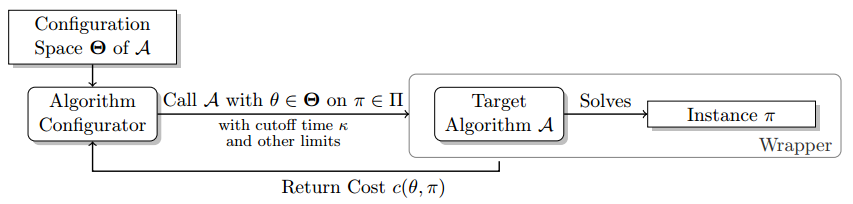
\includegraphics[width=\textwidth]{images/AC_workflow.png}
\captionsetup{justification=justified}
\caption[Algorithm configuration workflow]{Algorithm configuration workflow \cite{Pitfalls}. The target algorithm $\mathcal{A}$ is evaluated with different parameter configurations $\theta$ on various instances $\pi$ of the problem. The cost metrics of the evaluation $c(\theta,\pi)$ is provided to the configurator.}
\label{Fig:ACworkflow}
\end{figure}

The workflow of algorithm configuration is illustrated in figure \ref{Fig:ACworkflow}. Initially, the target algorithm $\mathcal{A}$ is executed by the configurator to solve a particular problem instance using a valid configuration $\theta$ \cite{Pitfalls}. The configuration space, $\Theta$ is used to sample the valid configuration. The target algorithm is optimized for the cutoff time $\kappa$ and other resource limitations such as memory consumption provided by the user at the time of execution. In order to preserve the generality of algorithm configuration procedures and optimize a wide range of target algorithms, wrappers are utilized. The wrapper runs the target algorithm and returns the cost metric to the configurator. The input to the wrapper is the input configuration and instances for evaluating the algorithm. The possible cost metrics or the performance metrics an algorithm configurator can optimize are runtime, solution quality, memory requirement, and error value. In contrast to runtime and memory, the solution quality optimization is a maximization problem.

With regard to this research work, the variables corresponding to the workflow of the algorithm configuration problem is defined in table \ref{Research_variables}.

\begin{table}[ht!]
\centering
\begin{tabular}{||c|c|c||} 
\hline
Variables & Variable name & Research resemblance \\ [0.5ex] 
\hline\hline
$\mathcal{A}$ & Target algorithm &Multiphysics simulation- FSI study \\ 
\hline
$\theta$ & Parameter configuration& Parameters of the coupling tool \\
\hline
$\Theta$ & Configuration space& Vector space spanned by the parameters \\
\hline
$\pi $& Problem instance & Single simulation instance \\
\hline
$\Pi $& Set of problem instances & Set of simulation instances \\
\hline
c & Performance metric & Runtime of the simulation (in seconds) \\
\hline
- &Wrapper & Command-Line Interface \\ [1ex] 
\hline
\end{tabular}
\captionsetup{justification=justified}
\caption[Research variables]{Research variables.}
\label{Research_variables}
\end{table}

\subsection{AAC mindmap}
\label{section:AACmindmap}
AAC effectively solves a wide range of target algorithms, namely Boolean satisfiability, mixed integer programming, configurable software systems, and machine learning algorithms. In addition, the performance metrics AAC algorithms focus to optimize is solution quality, run-time, memory requirements, approximation error, and plan length. The two major paradigms of algorithm configuration based on the approaches are model-based and model-free. The next chapter \ref{chapter:stateoftheart} provides an extensive overview of the various model-based in section \ref{section:model-based} and model-free in \ref{section:model-free} approaches implemented in AAC.

One of the imperative requirements for choosing the suitable AAC approach to a specific problem depends on the parameter types and the number of parameters involved in the study. With developments in the field of AAC, the state-of-the-art algorithms accommodate four types of parameters, namely categorical, numerical, and conditional. The categorical parameters are variables accepting discrete domain values and subdivided into three types. The three types of categorical parameters are dichotomous, ordinal, and nominal variables accepting binary, ordered, and unordered domain values. The numerical parameters include real or integer values. The discrete and continuous parameters are different types of numerical parameters \cite{parameter_types}. The conditional parameters refer to parameters dependent on a parent parameter. The conditional parameters are active in a configuration given the parent parameter is assigned to a specific value. The conditional parameters often denote a sub-process or parameter behaviour dependent on another process or parameter. 

The mindmap in figure \ref{fig:AAC_mindmap} illustrates the semantics of the field AAC.
 
\label{section:AAC-mindmap}

\begin{figure}[!ht]
\centering
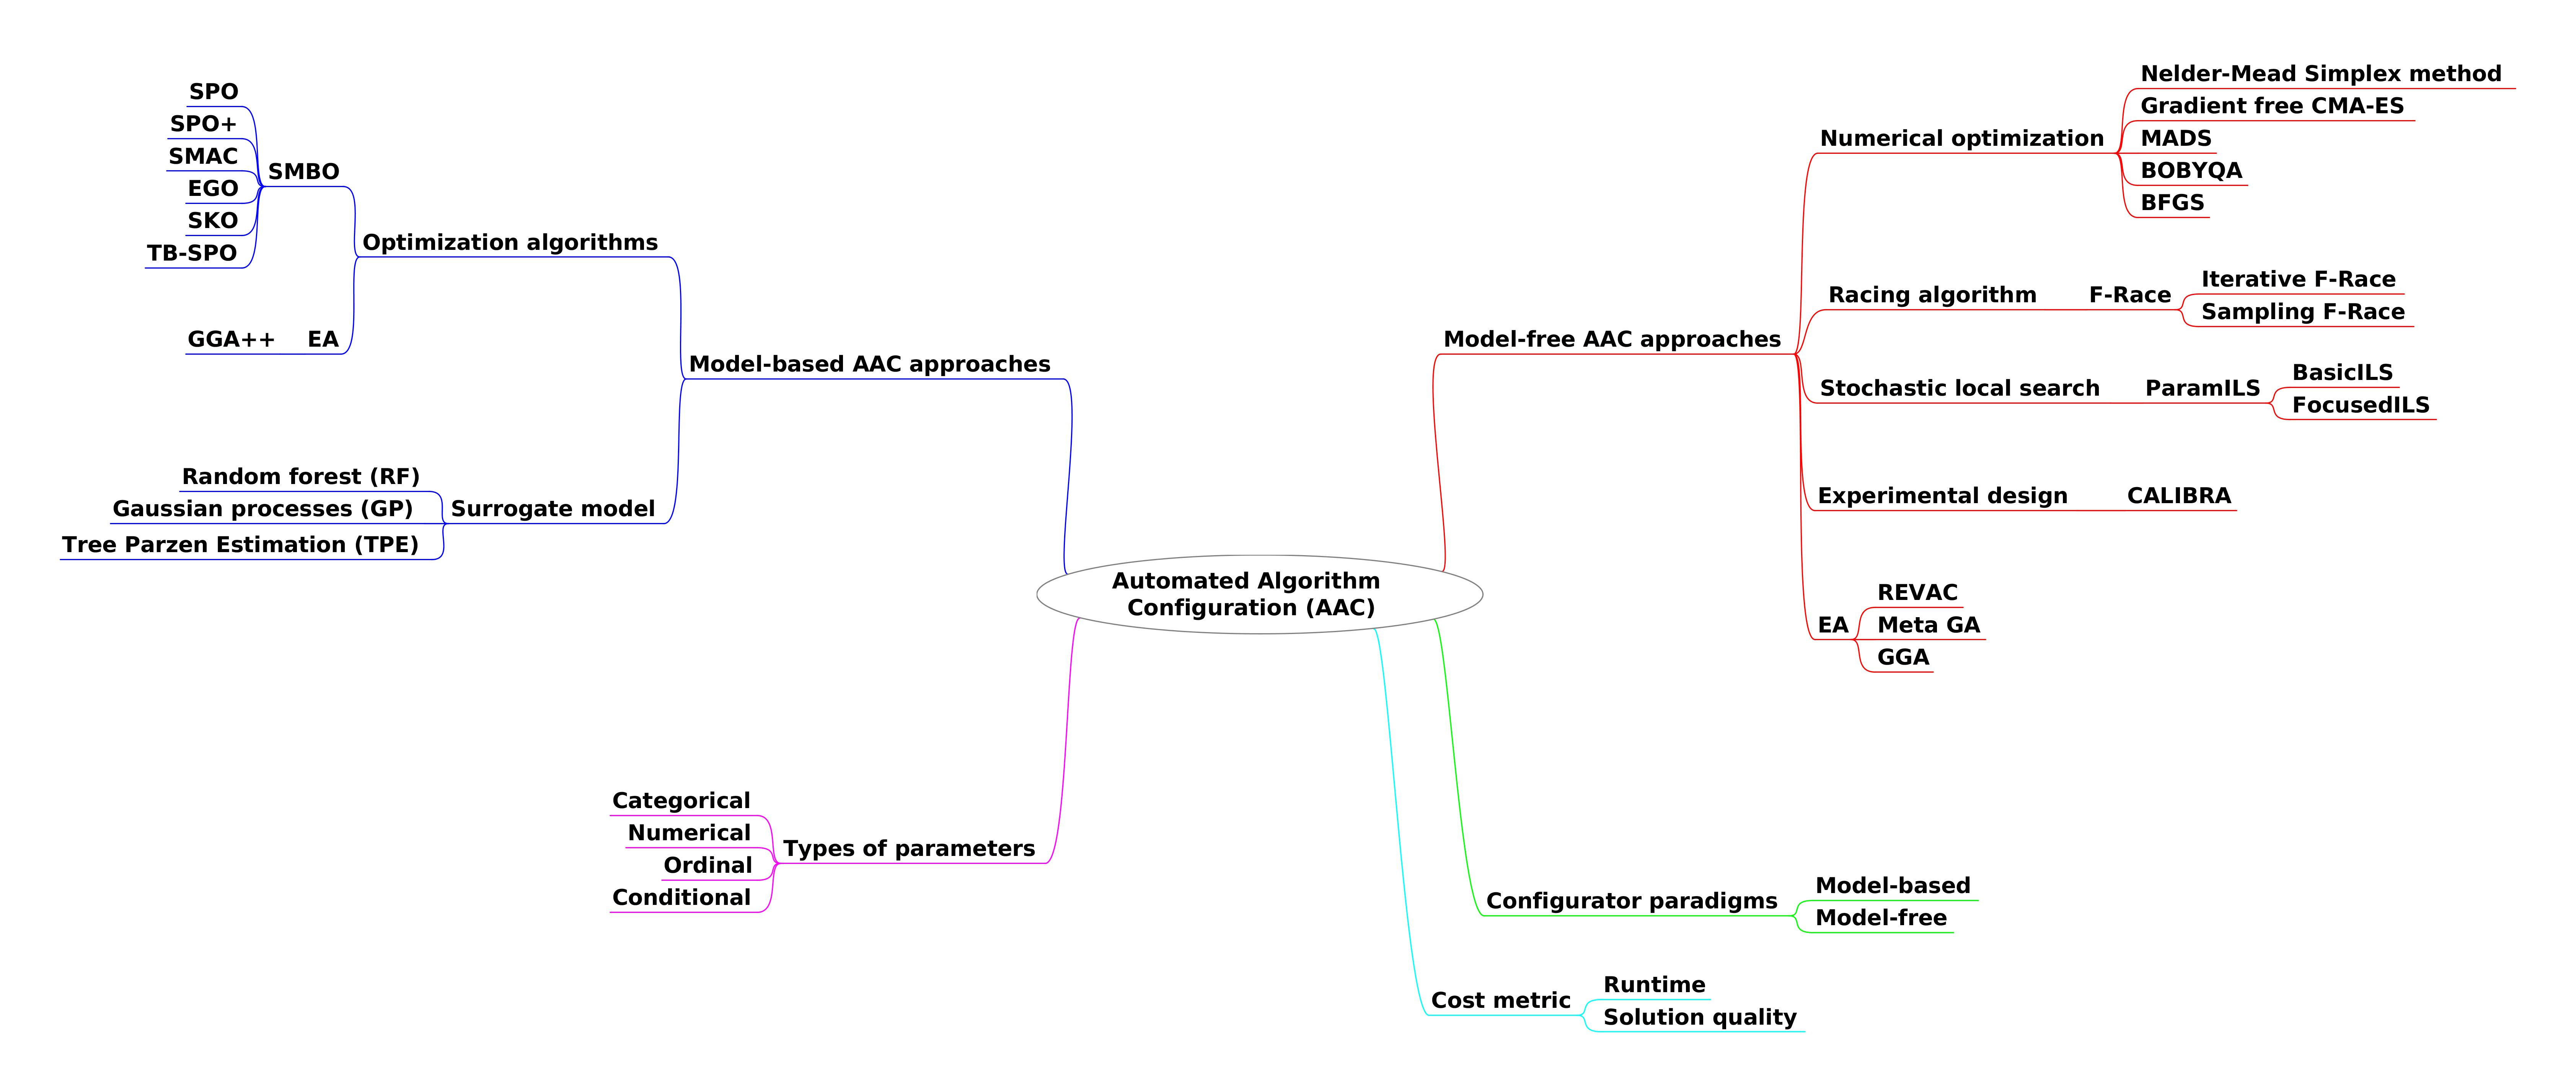
\includegraphics[width=\textwidth]{images/AAC_mindmap1.jpg}
\captionsetup{justification=justified}
\caption[Mindmap of Automated Algorithm Configuration]{Mindmap of Automated Algorithm Configuration.}
\label{fig:AAC_mindmap}
\end{figure}


\section{Bayesian Optimization (BO)}
\label{section:bayesianoptimization}

BO solves the mathematical problem of estimating the global maximum or minimum of an objective function, f. 

\begin{equation}
    \theta^* = \underset{\theta\in\Theta}{\text{arg max }} f(\theta) 
\end{equation}

$\Theta$ is the configuration space. $\theta$ is a parameter configuration of the black-box function f.  The information regarding the function structure such as concave or linear is unknown, and the function lacks the analytical expression to calculate gradient information \cite{BayesianOptimization_papertutorials}. However, evaluations can be performed at any valid query point $\theta$ from the domain. The output value of the function, y $\in$ R, is stochastic with noise. This serves as the minimum condition for BO \cite{Bayesianoptimization_review}.

BO is useful in optimizing expensive, multimodal, and non-convex objective functions. For instance, consider an image classification system f with hyperparameters x. A few tunable parameters 'x' of a deep network are learning rate, number of intermediate hidden layers and number of hidden layer neurons. The classification accuracy on a particular dataset is the evaluation result, y = f(x). The process of tuning the hyperparameters to maximize y is expensive because of the high evaluation cost of the function f. In this scenario, BO aids to effectively guide the search of optimal parameters and maximize y by estimating the optimal set of parameters x \cite{Bayesianoptimization_review} \cite{BayesianOptimization_papertutorials}. 

The applications of BO includes hyperparameter optimization of neural networks \cite{hponn}, gait optimization for legged robots \cite{robotgait}, and mixed-integer programming solvers \cite{SMAC_mainpaper}. In recent extensions of BO, the acceptable input variables are conditional, categorical and numerical \cite{SMAC_mainpaper} \cite{Bayesianoptimization_review} \cite{BayesianOptimization_papertutorials}.


The fundamental principle of BO is Bayes theorem. A probabilistic model (P(cost $\vert$ hyperparameters)) is constructed using the known prior belief of the objective function evaluations. This model is called the surrogate model. The prior distribution, P(c) is the set of costs for the initial samples/parameters obtained by evaluating the parameters on the objective function $R_n$= \{$(\theta_1,c_1),(\theta_2,c_2),...(\theta_n,c_n)$\}. The likelihood estimate of observing the data given the prior is estimated, $P(R_n|c)$. The surrogate is constructed using the below equation.

\begin{equation}
Posterior \propto Likelihood \times Prior
\end{equation}

\begin{equation}
P\left(c | \mathcal{R}_{n}\right) \propto P\left(\mathcal{R}_{n} | c\right) P(c)
\end{equation}


The posterior probability is the surrogate model. This conditional probability depicts the objective function performance $c=f(\theta)$, given the samples or parameter configuration is an estimation of the objective function performance. The surrogate model efficiency in summarizing the objective function is proportional with the evaluation count of the objective function with various configurations. In addition, the model aids to select the promising point for the upcoming evaluation. The selection is based on an acquisition function. This guide the search efficiently by decreasing the direct evaluation count of the objective function \cite{Bayesianoptimization_review} \cite{BayesianOptimization_papertutorials}. 

The query point is selected using the posterior surrogate model and the acquisition function. The surrogate model exploitation and exploration is mediated by the acquisition function. The former focus on the query point with the extreme value of the objective function and the latter estimate the query point with maximum uncertainty \cite{Bayesianoptimization_review} \cite{BayesianOptimization_papertutorials}. The new evidence is collected by evaluating the objective function at the new query point. The evidence is used to refine the model and update the posterior probability again. This is the basic principle behind all variants of Sequential Model-Based Optimization (SMBO) and the algorithm is provided in Algorithm 1 \cite{BayesianOptimization_papertutorials}. The initial function evaluations are carried out using arbitrary query points.


The algorithm of BO performs the following steps.

\begin{enumerate}

\item \textbf{Select initial sample:} Select sample points to query the noisy objective function and evaluate the points on the objective function. The figure \ref{fig:BO_objective} shows the evaluation of two initial sample points.

\item \textbf{Fit surrogate:} The surrogate model is fit to the initial samples. The iteration 1 in figure \ref{fig:BO1} illustrates the curve fit to the initial samples. The surrogate model performs regression task to predict the performance or cost metric of the objective function given the configurations. The various surrogate models available are Gaussian Process (GP), Random Forest (RF), and Tree Parzen Estimator (TPE).

\item \textbf{Optimize acquisition function:} This step includes optimizing the acquisition function to obtain the next query point to evaluate the objective function \cite{BayesianOptimization_papertutorials}. The various objective functions available are expected improvement (EI), maximum probability of improvement (MPI), and entropy search (ES). In this example, EI is used to select the upcoming query point. The improvement function, I($\theta$) is the difference in the predictions by the surrogate model for a particular configuration $\theta$ and the current best configuration $\theta^+$ \cite{EI_proper}. The equation is positive for a particular configuration better than the existing best configuration.

\begin{equation}
\mathrm{I}(\mathbf{\theta})=\max \left\{0, f_{n+1}(\mathbf{\theta})-f\left(\mathbf{\theta}^{+}\right)\right\}
\end{equation}

The next query point is determined by the maximal value of the expected improvement given by the following equation \cite{EI_analytical}.

\begin{equation}
\mathbf{\theta}=\underset{\mathbf{\theta}}{\operatorname{argmax}} \mathbb{E}\left(\max \left\{0, f_{n+1}(\mathbf{\theta})-f\left(\mathbf{\theta}^{+}\right)\right\} | \mathcal{R}_{n}\right)
\end{equation}

where, $f(\theta^+)$ is the best performance metric at the particular iteration and $f(\theta)$ is the predictions by the surrogate for a particular configuration in the distribution $\theta$. An analytical closed form of the EI is calculated for different surrogate models \cite{EI_analytical} \cite{EI_proper}.

EI quantifies the utility of the configuration to provide better performance on the target algorithm. Therefore, the configuration with larger value of EI is selected for evaluation on the target algorithm. EI is calculated using the empirical mean and variance of the performance metric distribution in the surrogate model \cite{EI_analytical} \cite{EI_proper}. In addition, the score balances between the high uncertainty regions of the distribution and high performance metric. The acquisition function subplots of the figures \ref{fig:BO1}, \ref{fig:BO2}, \ref{fig:BO3}, \ref{fig:BO4}, \ref{fig:BO5}, \ref{fig:BO6}, \ref{fig:BO7}, \ref{fig:BO8} depicts this step. The minimization and maximization of a particular problem depends on the procedure involved in optimizing the acquisition function. The maximization of the negated acquisition function models the minimization problem.
\item \textbf{Evaluate target algorithm:} The objective function is evaluated using the sample or the configuration selected from the acquisition function. The surrogate model is fit again. This is the step of collecting new evidence and updating the posterior.
\item \textbf{Repeat:} Perform fit surrogate, optimize acquisition function and evaluate target algorithm step until the consecutive query points converge or a budget criterion is satisfied.
\item \textbf{Incumbent configuration:} After exploiting the budget criterion or achieving convergence, the best sample point or the parameter configuration is returned. This sample point is the minimum or the maximum of the objective function depending on the problem formulation.
\end{enumerate}

\begin{table}[]
\centering
\begin{tabular}{|l|l|}
\hline
\textbf{Symbol} & \textbf{Meaning} \\ \hline
$\Theta$ & Configuration space. \\ \hline
$\theta_i$ & $i^{th}$ parameter configuration from the configuration space, ($\theta \in \Theta$). \\ \hline
$c_i$ & Cost of the $i^{th}$ parameter configuration. \\ \hline
$\Theta_{inc}$ & Best configuration/ Maximum or minimum query point. \\ \hline
$R_n$ & Set of n parameter configurations and respective costs. \\ \hline
f & Objective function or target algorithm under optimization.\\ \hline
$m$ & Surrogate model- Gaussian process, Random forest. \\ \hline
$\alpha$ & Acquisition function. \\ \hline
\end{tabular}
\captionsetup{justification=justified}
\caption[Symbols used in the BO algorithm]{Symbols used in the BO algorithm (Algorithm \ref{algo:bayesianopt}).}
\label{table:BOsymbols}
\end{table}

The BO algorithm (Algorithm \ref{algo:bayesianopt}) is adapted from \cite{BayesianOptimization_papertutorials} \cite{Bayesianoptimization_review}.
\newpage
$\\$
\begin{algorithm}[H]
\LinesNumbered
\SetAlgoLined
\DontPrintSemicolon
\caption{Pseudo-code for Bayesian Optimization}
\label{algo:bayesianopt}
\KwIn{Surrogate model m, objective function f, acquisition function $\alpha$, Initial query points $\theta_{initial}$ = \{$\theta_1$, $\theta_2$,..., $\theta_n$\}}
\KwResult{Global Maximum query point}
$c_{initial}$ $\leftarrow$ f($\theta_{initial}$)\\
$R_n$= \{$(\theta_1,c_1),(\theta_2,c_2),...(\theta_n,c_n)$\}\\
m $\leftarrow$ FitModel($R_n$).\\
\For{$i$ = 1,2 ..j}{
Select new $\theta_{n+1}$ by optimizing acquisition function $\alpha$.\newline 
$\theta_{n+1}$ $\leftarrow$ $\underset{\theta\in\Theta}{\text{arg max }} \alpha (\theta,R_n)$\\
Query objective function to obtain $c_{n+1}$\\
Augment the data, $R_{n+1}$ $\leftarrow$ \{$R_n, (\theta_{n+1}, c_{n+1})$\}\\
m $\leftarrow$ FitModel($R_{n+1}$).\\
\Return{\text{Query point }$\theta_{inc}$ \text{with maximum} f($\theta$) \text{from} $R_{n+1}$}}
\end{algorithm}
\DecMargin{1em}
$\\$

% Advantages of BO:

% 1. Finds global extrema of objective functions that are expensive to evaluate.
% 2. Finds global extrema of objective functions with no closed form expression.
% 3. Finds global extrema of objective functions when evaluations are costly.
% 4. Continuous and discrete space objective function and parameters.
% 5. Based on bayes theorem. Robust to noisy function evaluations.
% 6. Less evaluations on the target algorithm. beacause target evaluation is costly.
% 7. # parameters <=20. BO is useful.

% Disadv: 
% 1. More samples for more dimension to search.
% 2. Depends on the surrogate model parameters.
% 3. BO surrogate depends on another optimization task for finding next good to evaluate.
\raggedbottom

\section{Machine Learning (ML) models}
\label{section:machine learning models}

The following ML models are used to perform regression (refer section \ref{section:training_phase}) in this work.

% \subsection{Logistic regression}

% Logistic regression is a statistical method commonly used for supervised classification tasks. However, logistic regression is primarily a regression model predicting the probability of a particular class given the input data. The logistic regression utilize the logistic sigmoid function to model the input data.
% \begin{equation}
% p\left(\mathcal{C}_{1} | x\right)=y(x)=\sigma\left(\mathbf{w}^{\mathrm{T}} \boldsymbol{x}\right)
% \end{equation}

% $x$ is the feature vector. $p\left(\mathcal{C}_{1} | x\right)$ is the posterior probability of class $C_1$ for a given feature vector. The posterior of class 2 is given by $p\left(\mathcal{C}_{2} | x\right)$= 1- $p\left(\mathcal{C}_{1} | x\right)$. w is the weight associated with each feature and denotes the parameters of the regression model. The parameters are estimated by minimizing the cross-entropy error function using gradient descent. The decision boundary is linear and requires fewer parameters to model the training set compared to Gaussian Process (GP) \cite{Bishop_ML_book}. 

% The other ways of performing logistic regression is formulating the linear model by the inverse of the logistic function called logit function given by the natural logarithm of the odds of success.

% Refer LA slide- 06-LinearDiscriminant.
% https://www.gormanalysis.com/blog/logistic-regression-fundamentals/
% https://towardsdatascience.com/logit-of-logistic-regression-understanding-the-fundamentals-f384152a33d1

\subsection{K-Nearest Neighbors (KNN)}

KNN is a non-parametric supervised learning algorithm. The test samples are predicted depends on the K nearest training samples in the feature space provided. For classification, the output prediction is the majority vote of the K nearest samples class membership in the training examples. For regression, the mean of the K nearest samples is the dependent variable value. The algorithm is sensitive to the K value and model is slower on increasing data volume \cite{KNN}. The majority vote is affected in a skewed distribution of classes. One of the ways to mitigate the issue is to assign a weight value to each data point depending on the distance from the test sample \cite{scikit-learn}.

\subsection{Support Vector Machine (SVM)}

SVM is a supervised learning machine for classification and regression tasks \cite{SVM_tutorials}. For classification, SVM estimates the optimal decision boundary or hyperplane with maximum margin of separation between different classes. The distance between the hyperplane and the data samples on both sides of the hyperplane is called the margin. SVM finds an optimal decision boundary for linearly separable data. However, SVM supports linearly non-separable data by using a kernel trick. The kernels are functions projecting the low dimensional input features to high dimensional features. This kernel functions transform a linearly non-separable data in lower dimension into linearly separable data in higher dimension. Polynomial, Radial Basis Functions (RBF) and sigmoid are popular kernel functions. The support vectors are the critical points exactly at the margin of separation on either side. The support vectors affect the position of the hyperplane. The optimal decision boundary is estimated by minimizing an error function with constraints. The decision y for a particular feature x is given by, $y = sign(w.x + b)$. w and b are parameters of the decision boundary. For regression, $y = w.x +b$ provides the target variable value \cite{SVM_tutorials}.


\subsection{Random Forest (RF)}

RF is an ensemble based classification and regression machine learning model building numerous decision trees. RF utilizes a bootstrap sampling process for selecting the training set by random sampling with replacement called bagging. In addition, RF selects random subset of the available features for splitting the data at each node. Among the subset of features, the features for splitting the samples depends on the information gain (IG) provided by the feature. The IG is a metric providing the amount of information provided by the feature regarding the class in classification tasks or prediction variable in the regression tasks. The feature with maximum information gain is selected for splitting the data at each node. A large value of IG represents less entropy in the resulting data groups after split.  In classification task, each tree predicts the label class and the class with maximum vote is assigned to the test data. In regression task, each tree predicts the response dependent variable and the average of the prediction across all trees is the test data value. RF reduces the overfitting issue of decision trees by injecting randomness in the process through bootstrap aggregation, feature bagging and averaging the result of numerous trees \cite{RF_book} \cite{RF_mainpaper}.
%  Increases bias little and reduces variance of the model.
% This technique is called feature bagging or bagging
\subsection{Quantile Random Forest (QRF)}

QRF performs quantile regression and the process of building a tree is exactly similar to random forest. The significant difference between QRF and RF is all the information regarding the target variable is preserved after training instead of averaging the target variable value at a particular leaf node. All the target variable values at a particular leaf are used in the prediction phase to predict at a particular quantile value. For instance, the leaf node of any particular tree after training hold the values - 1,2,3,4, and 5, the prediction at 25 percentile is 2. In constrast to RF predicting conditional mean, this type of quantile regression provides the conditional quantiles \cite{QRF} \cite{scikit-learn}.


% Quantiles are values of the sample set dividing the values into equal sized groups. 10\% quantile is 5 means, 10\% of the samples are less than the value 5. Percentile are quantiles that divide the data into 100 equally sized groups.
% Quantiles and percentiles are used when we divide the samples into its own group. 0 percentile or quantile is the sample value below which there is no samples.
% Quantile regression states the values of a features set at particular quantile. 
% Can use quantile regression to predict without  outliers in the range 98.75, calculate prediction interval of a prediction given in (https://blog.datadive.net/prediction-intervals-for-random-forests/)
% https://www.youtube.com/watch?v=IFKQLDmRK0Y =>Quantile regression
% https://www.youtube.com/watch?v=AnOTOFuC6ZM
% https://support.sas.com/resources/papers/proceedings17/SAS0525-2017.pdf => SAVE PDF and IMAGE to explain the importance of capturing the conditional variance.


\subsection{Gradient Boosting Machines (GBM)}

GBM is an ensemble method of building weak classifiers in a sequential manner. Each of the week classifiers predict the training labels with atleast 50 percentage accuracy. Initially, a weak model is assigned with a constant value (average of the target variable). Secondly, a GBM fits a weak classifier to the training features with the the pseudo-residual error calculated by the negative gradient of the user-defined error function. The weight of the weak classifier depends on the target and the aggregate prediction of the existing weak classifiers solved using an one-dimensional optimization task. The weak classifiers are built in an additive manner until the pseudo-residual reaches a tolerance. GBM is a variant of Adaboost with a differential error function optimized using steepest descent. In contrast, Adaboost increases and decreases the weight of the wrongly and correctly classified data sample respectively in the next weak classifier. The final classifier is an aggregation of the each weak classifier output \cite{GBM} \cite{Bishop_ML_book}.

\section{Metrics}

The following metrics are utilized in the experiments and results (chapter \ref{chapter:experimentation_results}) to evaluate the proposed strategy and the ML models.

\subsection{Statistical dispersion}
The following statistical metrics quantify the spread of a distribution. The repeatability coefficient is estimated using the common dispersion metrics.
\subsubsection{Variance and Standard deviation}
Variance is based on the measure of deviation of individual samples from the mean \cite{statistic_definition}. It is the mean of the squared difference of each sample from the mean given by the equation \ref{equation:variance}. $x_i$ is the $i^{th}$ sample in the data, n is the total number of samples in the data and $\mu$ is the mean of all the samples in the data. The denominator (n-1) provides an unbiased estimate of the population variance and population standard deviation from the respective sample statistics.

\begin{equation}
\sigma^{2}=\frac{\sum_{i=1}^{n}(x_i-\mu)^{2}}{n-1}
\label{equation:variance}
\end{equation}

\begin{equation}
\text{standard deviation},\sigma=\sqrt{\frac{\sum_{i=1}^{n}(x_i-\mu)^{2}}{n-1}}
\label{equation:standarddeviation}
\end{equation}

\subsubsection{Repeatability coefficient}
\label{section:repeatability_coeff}
Repeatability coefficient, $S_r$ is given by the equation \ref{equation:repeatabilitycoefficient}. The maximum deviation with a probability of 95\% between two successive measurements of the same subject under same measurement conditions and using the same procedure \cite{repeatability1} \cite{repeatability2}.

% http://qibawiki.rsna.org/images/8/8c/FMRITechnicalPerformanceIndices041613.pdf
%  https://obgyn.onlinelibrary.wiley.com/doi/full/10.1002/uog.5256
% https://en.wikipedia.org/wiki/Repeatability
%  https://www-users.york.ac.uk/~mb55/meas/ba.pdf
\begin{equation}
S_r = 1.96 \times \mathrm{\sigma}
\label{equation:repeatabilitycoefficient}
\end{equation}

The standard deviation, $\sigma$ is the within group standard deviation. The reason is repeatability focus on the agreement of run-time on a particular instance and the deviation between different instances are avoided. In certain literature \cite{repeatability_final}, a multiplication factor $\sqrt{2}$ is included in the above equation \ref{equation:repeatabilitycoefficient} and provides an over estimate of the repeatability coefficient. Therefore, the equation \ref{equation:repeatabilitycoefficient} is used in this project \cite{repeatability_final} \cite{repeatability_final2} \cite{repeatability_final3}. The within-group standard deviation is computed using Analysis of Variance (ANOVA). 

"ANOVA is a statistical technique to analyze significant differences between mean of different groups. In one-way analysis of variance, the statistically significant differences between the means of three or more independent groups is tested" \cite{anova} \cite{anova2}. The assumptions of ANOVA include parametric and normally distributed data \cite{anova}. ANOVA estimates F-statistics or F-ratio. F-ratio signifies the differences in the sample mean. A less F-ratio signifies the samples are more similar. The two hypothesis in ANOVA are null and alternate hypothesis. The F-statistics and p-value from ANOVA are used to accept the null hypothesis or reject the null hypothesis. Null hypothesis and alternate hypothesis is stated in equation \ref{equation:hypothesis}. $\mu_g$ and $\mu_m$ are the sample means of any two groups in the observation. $\mu_i$, where i = 1,...N is the sample means of the N groups in the observations \cite{anova}. 

\begin{equation}
\begin{array}{ll}{\boldsymbol{H}_{o}: \boldsymbol{\mu}_{1}=\boldsymbol{\mu}_{2}=\cdots=\boldsymbol{\mu}_{N}} & {\text { Null hypothesis }} \\ {\boldsymbol{H}_{1}: \boldsymbol{\mu}_{g} \neq \boldsymbol{\mu}_{m}} & {\text { Alternate hypothesis }}\end{array}
\label{equation:hypothesis}
\end{equation}


\begin{equation}
\mathrm{F}=\text { Between group variability / Within group variability }
\end{equation}

\begin{equation}
\begin{aligned} F &=\frac{M S_{b}}{M S_{w}}  \end{aligned}
\end{equation}

$MS_b$ and $MS_w$ is the mean of square differences between and within groups of a sample \cite{anova}.

\begin{equation}
\begin{aligned} MS_{b} &=\frac{S S_{b}}{df_b}  \end{aligned}
\end{equation}
% https://stats.stackexchange.com/questions/50727/f-statistic-f-critical-value-and-p-value
\begin{equation}
\begin{aligned} MS_{w} &=\frac{S S_{w}}{df_w}  \end{aligned}
\end{equation}

The denominators $df_b$ and $df_w$ are the degrees of freedom between groups and within group described in equation \ref{equation:withindf} and \ref{equation:betweendf}. N is the total samples in the data without considering the groups. K is the total groups \cite{anova}. 

\begin{equation}
\begin{aligned}
df_{w} = N-K
\end{aligned}
\label{equation:withindf}
\end{equation}

\begin{equation}
\begin{aligned}
df_{b} = K-1
\end{aligned}
\label{equation:betweendf}
\end{equation}

\begin{equation}
\begin{aligned}  SS_{b}=& n_{k} \sum_k\left(\bar{x}_{k}-\bar{x}_{G}\right)^{2} \end{aligned}
\end{equation}

$SS_b$ is the between group sum of squared differences representing the total variability between the average of different groups \cite{anova}. 

\begin{equation}
\begin{aligned} SS_{w} &=\sum_i\left(x_{i}-\bar{x}_{k}\right)^{2} \end{aligned}
\end{equation}

$SS_w $ is the within-group sum of squared differences. $\bar x_G$ is the total mean of all the observations in the dataset. The mean of each group is $\bar x_k$.  $x_i$ is the value of a specific sample, i in the group \cite{anova}.

% \subsection{Classifier performance metrics}

% \subsubsection{Accuracy}

% Accuracy is the ratio of number of correct classifications to the total number of data points classified. True positive ($T P$) represents the positive prediction of a positive sample by the classifier model. True negative ($T N$) represents the negative prediction of a negative data point by the model. False positive ($F P$) represents the negative prediction of a positive data point by the model. False negative ($F N$) represents the positive prediction of a negative datapoint by the model. Therefore, $T P$ and $T N$ are correct predictions by the classifier. In contrast, $F P$ and $F N$ are wrong predictions by the classifier. Accuracy is a good metric on a balanced dataset.

% \begin{equation}
% \text { Accuracy }=\frac{\text{Number of correct predictions}}{\text{Total number of predictions}} = \frac{T P+T N}{T P+T N+F P+F N}
% \end{equation}

% \subsubsection{Precision}

% Precision provides the ratio of positive samples correctly classified to the total positive samples in the test set. It is a measure of exactness of the classifier.
% \begin{equation}
% \text { Precision }=\frac{T P}{T P+F P}
% \end{equation}

% "What proportion of positive predictions by the classifier model is actually positive?" \cite{GoogleML-course}. The model predicting zero $F P$ has a precision value 1.

% \subsubsection{Recall}

% Recall provides a measure of positive samples correctly classified to the total positive predictions by the classifier model. It is a measure of completeness of the classifier and called sensitivity.

% \begin{equation}
% \text { Recall }=\frac{T P}{T P+F N}
% \end{equation}

% "What proportion of actual positive sample is predicted correctly by the classifier model?" \cite{GoogleML-course}. The classifier model predicting zero $F N$ has a recall value 1.

% \subsubsection{F1 score}

% F1 score provides a balance between precision and recall taking note of the false negative and false positives. It is a better metric than accuracy in imbalanced datasets. 

% \begin{equation}
% \mathrm{F} 1=2 \times \frac{\text { Precision } \times \text {Recall}}{\text { precision }+\text {Recall}}
% \end{equation}


\subsection{Regressor performance}

The regressor models are compared using the following error metric in experiment \ref{section:trainingexperiment}.

\subsubsection{Root Mean Square Error (RMSE)}
\label{section:rmse_metric}
RMSE provides an estimation of the residual standard deviation. RMSE is the square root of the average of squared difference between the predicted and true values \cite{sklearn_api} \cite{scikit-learn}. It provides more error weightage to the larger errors. RMSE criticise larger error values more compared to the smaller errors \cite{sklearn_api} \cite{scikit-learn}. The error holds the same units of the estimated quantify. In addition, it overcomes the under-estimation issue of MSE for error values lesser than 1 by providing error in the same units of the quantified variable. RMSE is provided in equation \ref{equation:rmse}. $y_j$ and $\hat y_j$ represents the actual and predicted values of a set of 'n' samples \cite{sklearn_api} \cite{scikit-learn}. 
\begin{equation}
\mathrm{RMSE}=\sqrt{\frac{1}{n} \sum_{j=1}^{n}\left(y_{j}-\hat{y}_{j}\right)^2}
\label{equation:rmse}
\end{equation}



% https://stats.stackexchange.com/questions/27951/when-are-log-scales-appropriate
% https://www.aaai.org/Papers/JAIR/Vol32/JAIR-3214.pdf
% https://stats.stackexchange.com/questions/18844/when-and-why-should-you-take-the-log-of-a-distribution-of-numbers
% https://datascience.stackexchange.com/questions/40089/what-is-the-reason-behind-taking-log-transformation-of-few-continuous-variables

% \section{Dimensionality reduction techniques}

% \subsection{Principal Component Analysis (PCA)}
% The PCA projects the data into lower dimension providing the principal components with high variance in the data. It is a linear transformation dimensionality reduction method. The data is normalized before applying PCA because the dataset has different units. The normalization makes the features comparable and reduces the deviation in the data. This provides reasonable covariance between the features without bias due to scales and thereby provides PCA without bias in the features \cite{Bishop_ML_book}.

% \subsection{t-distributed Stochastic Neighbor Embedding (t-SNE)}

% The t-SNE aids in visualizing high dimensional data in a lower dimension. In contrast to PCA, t-SNE focus on the local relationships between data points in the higher dimension. This feature aids in generating a low dimensional representational map with non-linear behavior. This two/three dimensional map is developed in two steps. Firstly, developing a probability distribution with higher probability and low probability to similar and dissimilar objects respectively depending on the near and distant points in the high dimensional space. In the second step, a mismatch metric, is minimized to generate a lower dimensional distribution similar to the high dimensional distribution \cite{t-SNE-original}.  

% Kullback-Leibler divergence- mismatch metric. Sometime euclidean norm is also used.






